\chapter{پیاده‌سازی}

در بخش قبلی معماری کلی سامانه و ماژول‌های موردنیاز برای پیاده‌سازی سامانه پایش شبکه بیان و به صورت اجمالی معرفی شدند. این فصل به چگونگی قرار گرفتن و ارتباط بخش‌های مختلف می‌پردازد و پیاده‌سازی سیستم را توضیح خواهد داد.


ماژول‌های تعریف شده در فصل قبل برای سامانه پایش شبکه‌های کامپیوتری را می‌توان در چهار دسته کلی قرار داد: 

\begin{itemize}
    \item هسته \lr{SNMP}
    \item واسط کاربری 
    \item سمت سرور
    \item ذخیره‌سازی اطلاعات


\end{itemize}

در ادامه برای هر دسته توضیحاتی ارائه خواهد شد. این توضیحات شامل ماژول‌های دربرگیرنده آن، بررسی راه‌های ممکن برای پیاده‌سازی هر ماژول و درنهایت نحوه پیاده‌سازی آن ماژول خواهد بود. 


\section{هسته \lr{SNMP}}

این دسته فقط شامل ماژول هسته \lr{SNMP} از \cref{fig.11} است. در این ماژول، هدف توسعه ابزاری است که بتوان از طریق آن انواع پیام‌های \lr{SNMP} را ارسال و دریافت کرد. بدین منظور با تعریف دو کلاس تله\LTRfootnote{\lr{Trap}} و نشست\LTRfootnote{\lr{Session}} این ماژول را پیاده‌سازی می‌کنیم. توجه شود که کتابخانه \lr{net-snmp} به زبان \lr{C} است ولی این ماژول جهت توسعه بهینه در زبان \lr{C++} توسعه داده شد. در نهایت ابزاری برای این ماژول تولید شد که قابلیت دریافت پیام‌های تله و همچنین ارسال و دریافت پیام‌هایی از نوع  \lr{get} و \lr{walk} را دارد\cite{Mirfendereski_Centom}.

\newpage

\section{واسط کاربری}

این دسته فقط شامل ماژول واسط کاربری تحت وب از \cref{fig.11} است. این قسمت برای توسعه بهینه همانطور که در فصل قبل گفته شد با چارچوب ری‌اکت توسعه داده شد. در این قسمت قدم به قدم واسط کاربری توسعه داده شده به همراه کارایی آن مورد بررسی قرار می‌دهیم\cite{Mirfendereski_Centom}.


در \cref{fig.12} و \cref{fig.13} فهرست امکانات سامانه نشان داده می‌شود که شرح مختصری از آن‌ها در ادامه آورده شده است:


\begin{figure}[!h]
    \centering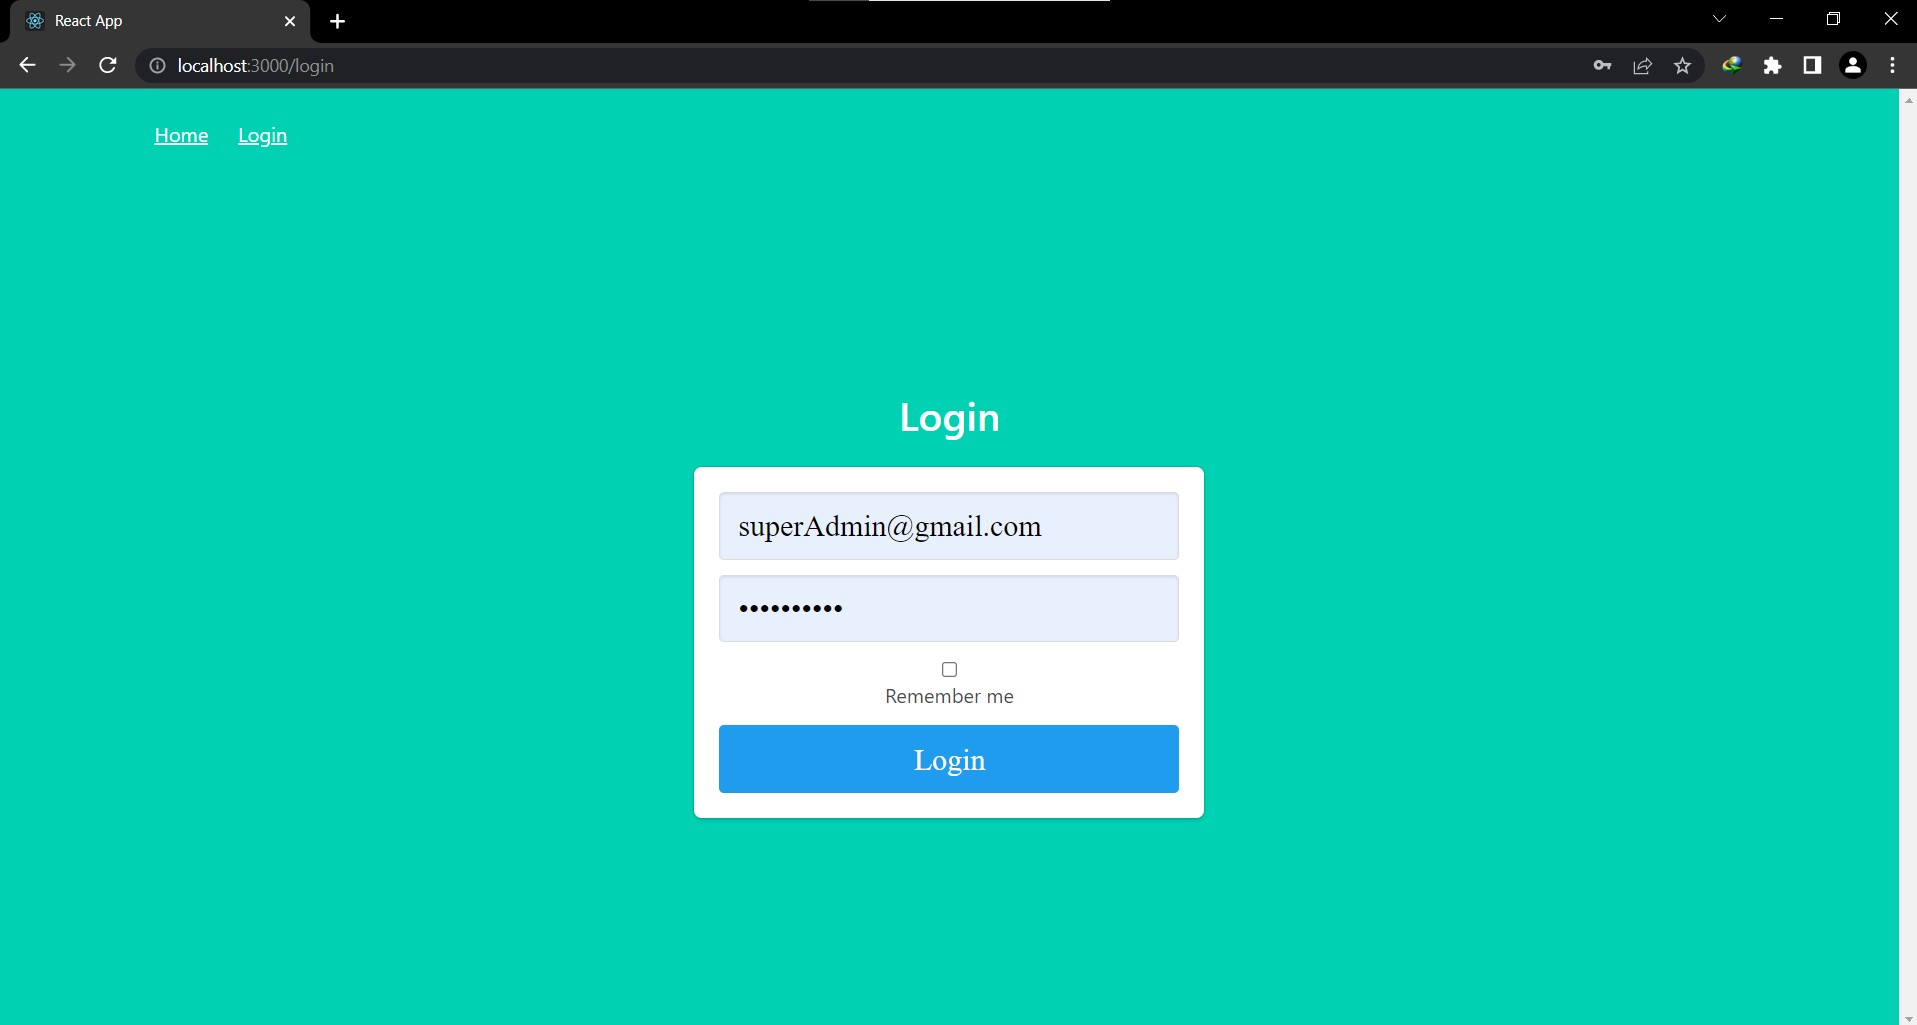
\includegraphics[scale=.38]{./nav-logout}
    \caption{فهرست امکانات سیستم هنگام ورود}\label{fig.12}
\end{figure}

\begin{figure}[!h]
    \centering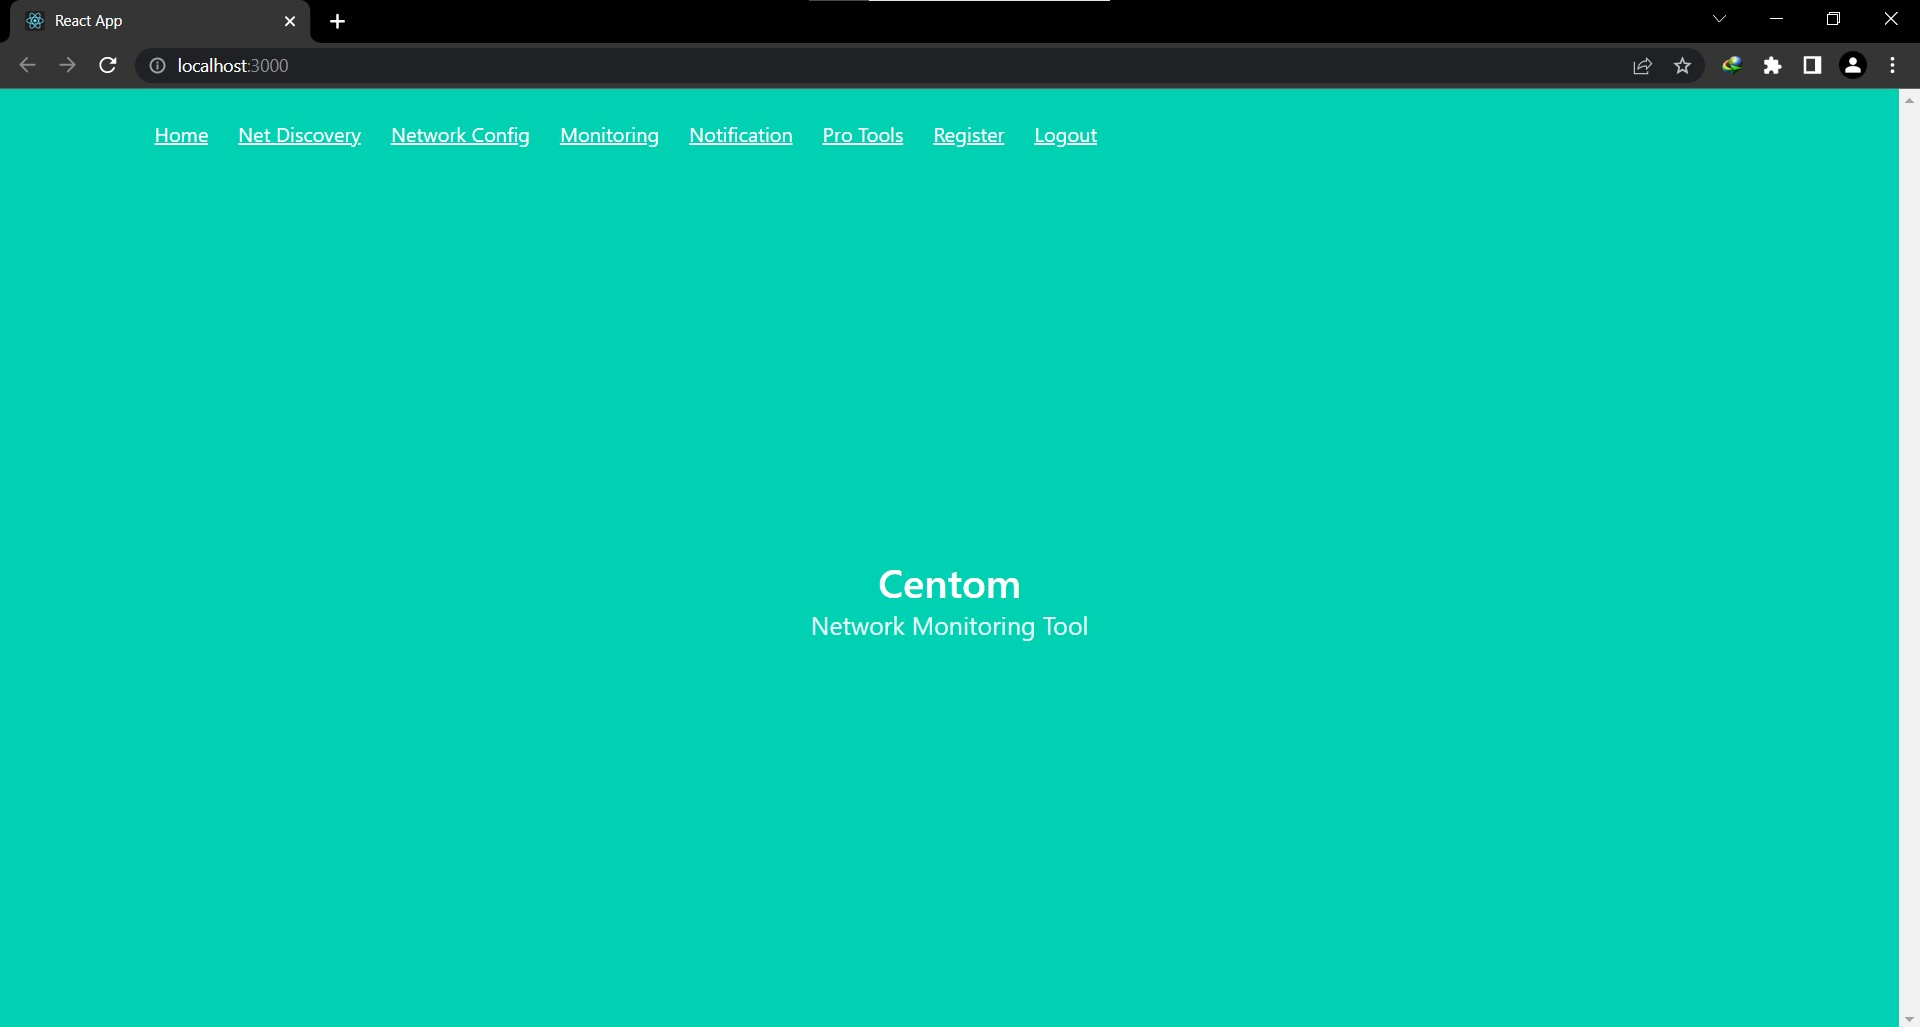
\includegraphics[scale=.38]{./nav-login}
    \caption{فهرست امکانات سیستم بعد از ورود مدیر ارشد}\label{fig.13}
\end{figure}
        
زمانی که کاربری وارد سیستم نشده است (\cref{fig.12})، تنها دو صفحه خانه و ورود به سامانه قابل دسترسی خواهد بود. این بدان علت است که در این سامانه ثبت‌نام\LTRfootnote{\lr{Register}} کاربر فقط توسط مدیر ارشد صورت می‌گیرد. در \cref{fig.13} فهرست امکانات پس از ورود مدیر ارشد نمایش داده شده‌اند. تاکیر بر روی مدیر ارشد بدین علت است که در این سامانه سه سطح دسترسی مدیر ارشد، مدیر معمولی و کاربر عادی وجود دارد. مدیر ارشد به همه امکانات دسترسی دارد. همچنین مدیر معمولی به ثبت‌نام کاربر جدید، تنظیمات و اسکن شبکه دسترسی ندارد. کاربر عادی نیز فقط به اسکن سریع یک دستگاه دسترسی خواهد داشت. البته لازم به ذکر است که سامانه یک مدیر ارشد دارد!

\newpage

تعریف کاربر جدید فقط توسط مدیر ارشد تحت صفحه ثبت‌نام در \cref{fig.14} ممکن خواهد بود. برای ثبت‌نام یک کاربر، مدیر ارشد ابتدا باید یک پست الکترونیکی\LTRfootnote{\lr{Email}} و رمز عبور وارد نماید. سپس باید برای سطح دسترسی بین دو نقش مدیر معمولی و یا کاربر معمولی انتخاب نماید. در نهایت نیز پست الکترونیکی و رمز عبور را در اختیار شخص متقاضی قرار می‌دهد.


\begin{figure}[!h]
    \centering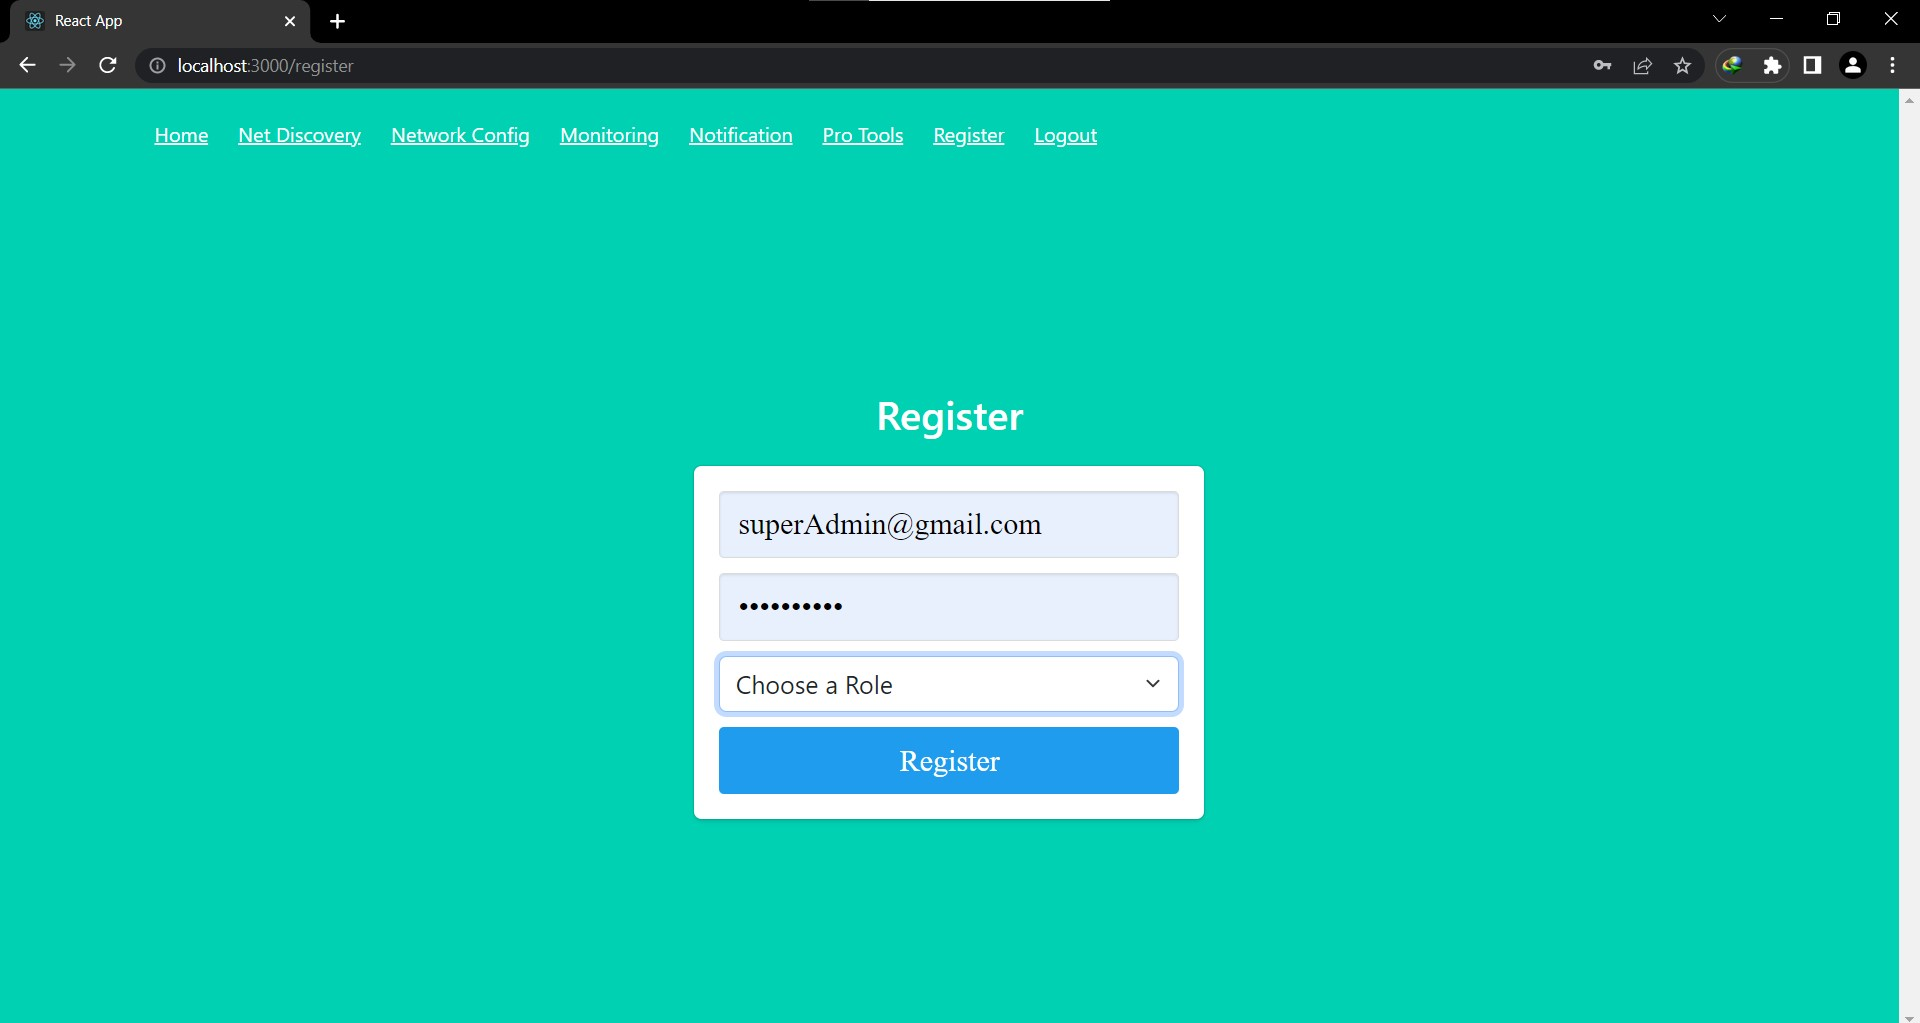
\includegraphics[scale=.35]{./register}
    \caption{صفحه ثبت‌نام در اختیار مدیر ارشد}\label{fig.14}
\end{figure}

\cleardoublepage

مهم‌ترین قسمت این سامانه، کشف شبکه است که اولین گزینه بعد از صفحه خانه قرار دارد. واسط کاربری این قسمت قبل و بعد از تست در \cref{fig.15} و \cref{fig.16} نشان داده شده‌ است. 


\begin{figure}[!h]
    \centering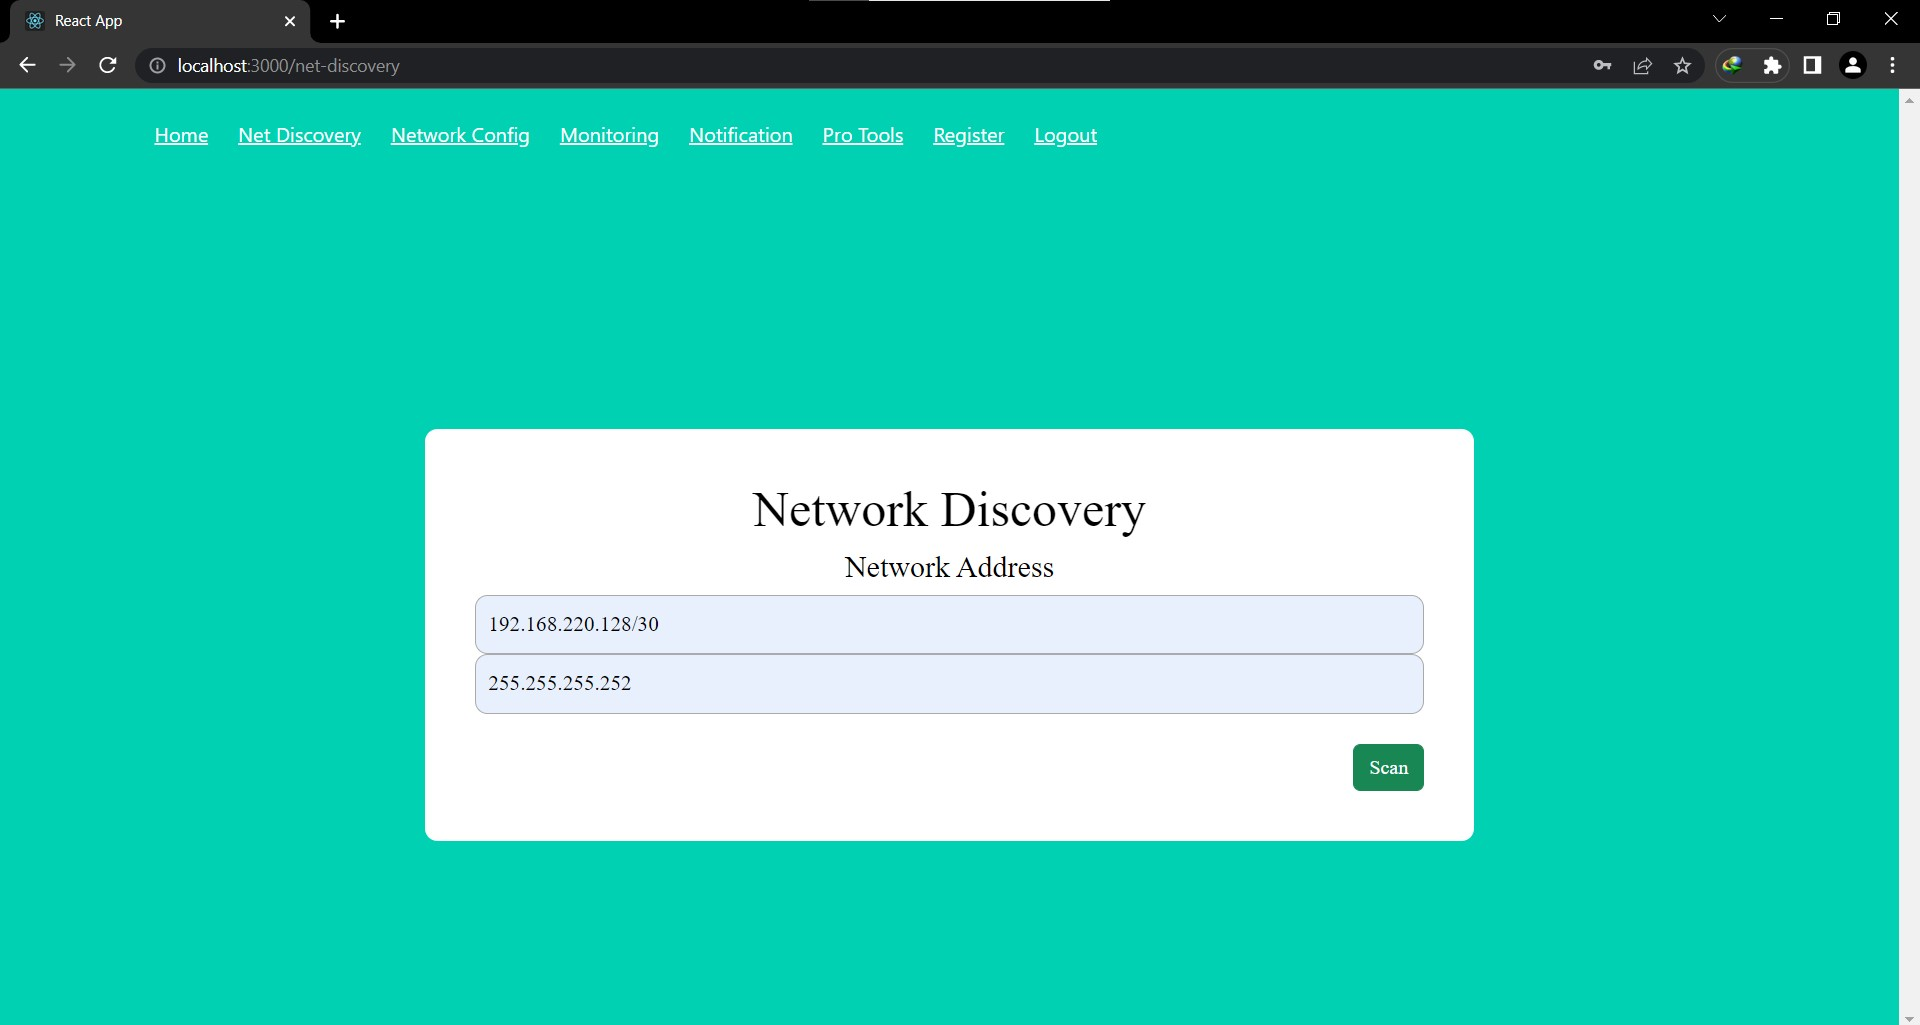
\includegraphics[scale=.38]{./net-dis-before}
    \caption{صفحه کشف شبکه قبل از اسکن}\label{fig.15}
\end{figure}


\begin{figure}[!h]
    \centering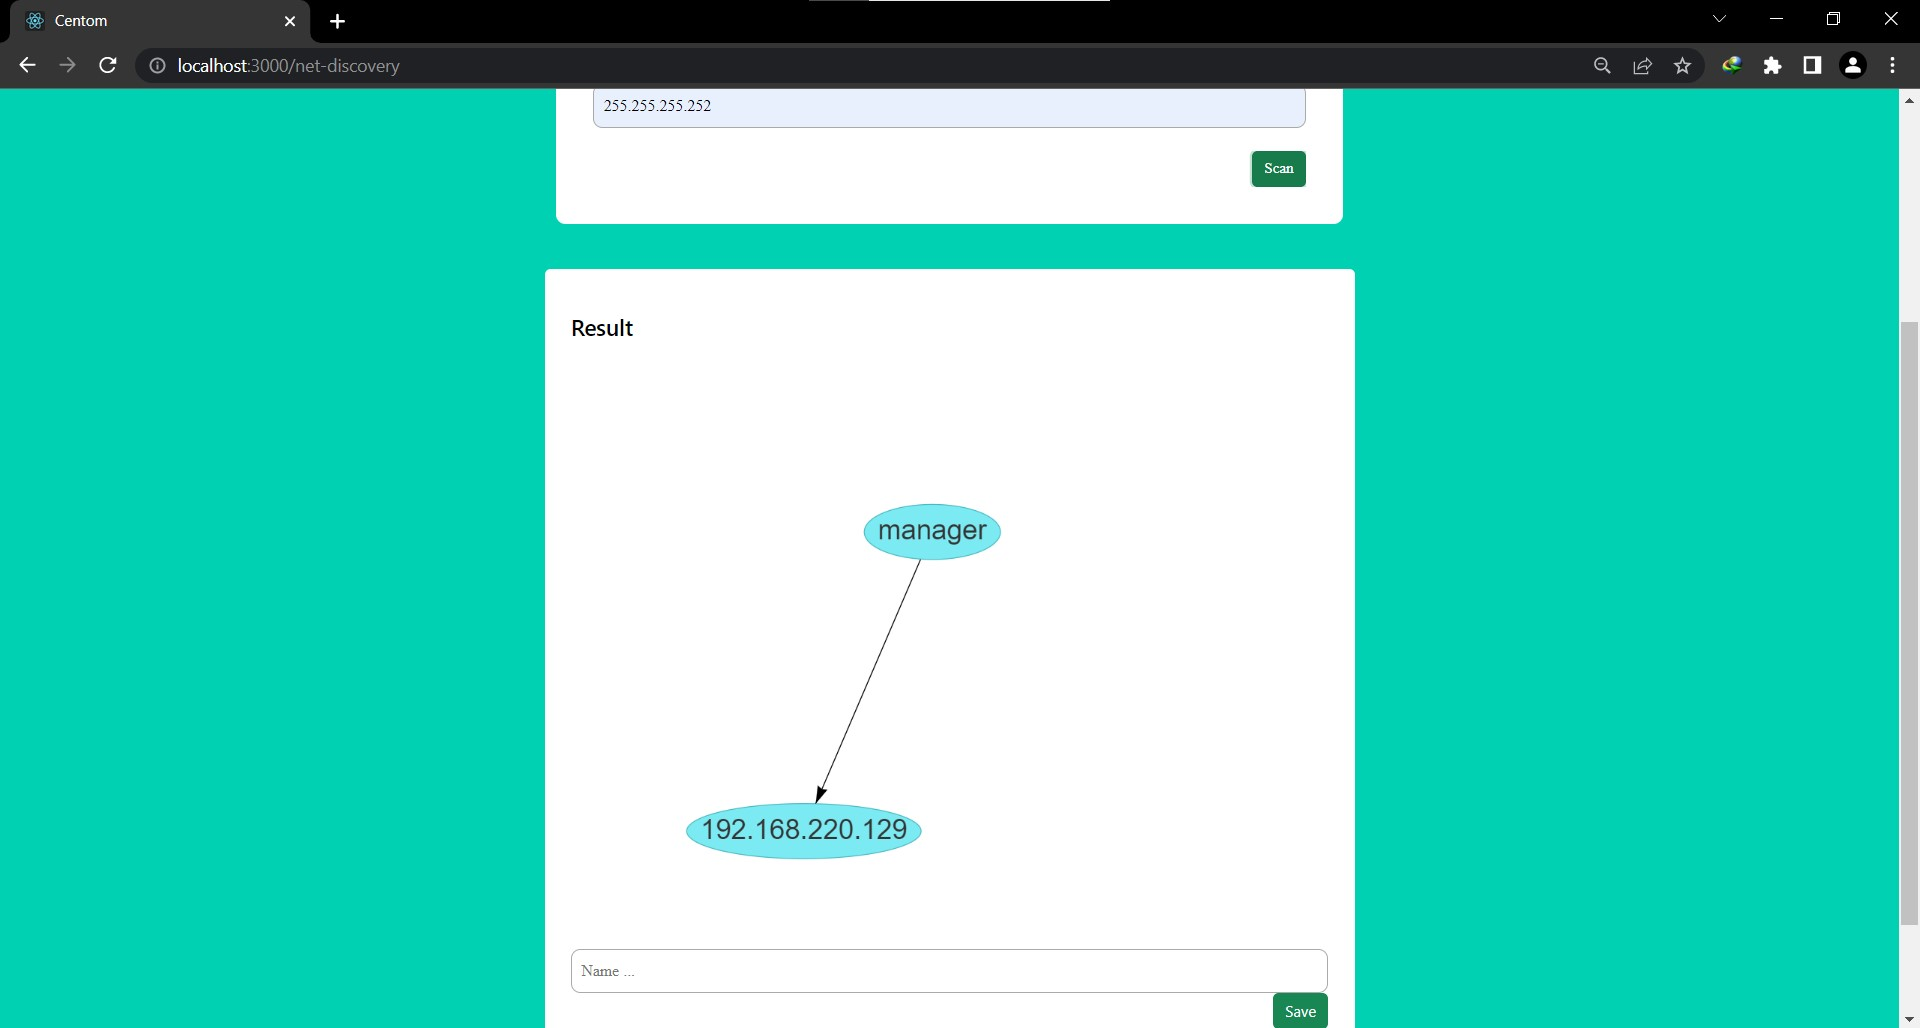
\includegraphics[scale=.38]{./net-dis-after}
    \caption{خروجی اسکن شبکه در قالب یک گراف}\label{fig.16}
\end{figure}

\cleardoublepage

در کشف شبکه ابتدا یک آدرس شبکه به همراه نقاب زیر شبکه\LTRfootnote{\lr{Subnet Mask}} از مدیر ارشد گرفته می‌شود. سپس بعد از اتمام اسکن شبکه، خروجی در قالب یک گراف نمایش داده می‌شود. درنهایت مدیر ارشد می‌تواند در صورت نیاز شبکه را با اسمی دلخواه در سامانه ذخیره کند.


بعد از ذخیره‌ سازی شبکه در قسمت قبل، مدیر ارشد می‌تواند ابتدا اطلاعات و تنظیمات شبکه را وارد نماید و بعد از آن اقدام به پایش شبکه کند. بدین ترتیب بعد از صفحه کشف شبکه، صفحه ذخیره تنظیمات شبکه در \cref{fig.17} وجود دارد. ابتدا با انتخاب اسم شبکه و نوع دستگاه‌های مورد نظر سامانه لیستی از آدرس‌ها را نشان می‌دهد. که با انتخاب یک آدرس مشخصات آن توسط کاربر وارد می‌شود. همچنین می‌تواند پارامترهای مورد نظر برای پایش دستگاه را به صورت لیست اضافه کند.



\begin{figure}[!h]
    \centering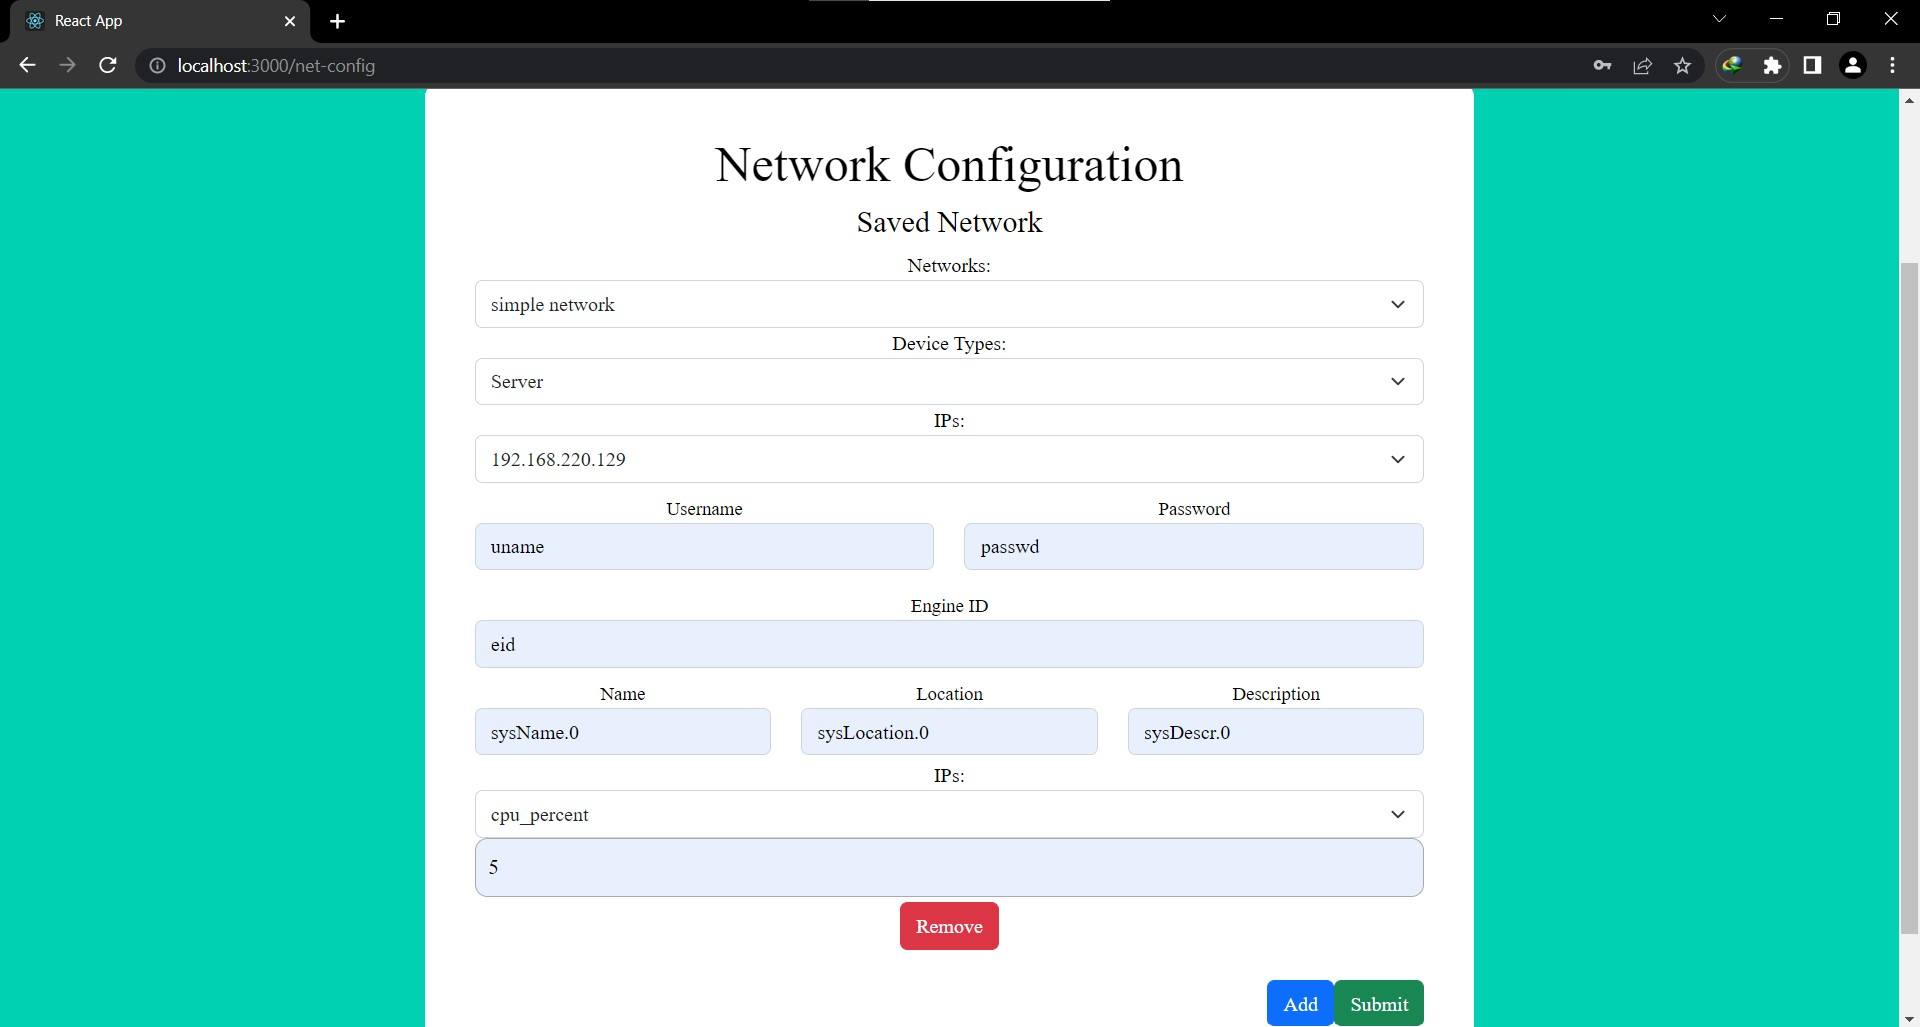
\includegraphics[scale=.38]{./net-config}
    \caption{صفحه ذخیره تنظیمات شبکه}\label{fig.17}
\end{figure}


% مانیتورینگ ///////////////////////////////////////////////////////////////////////////////////////////////////////
بعد از دریافت تنظیمات شبکه در مرحله قبل حال نوبت به پایش شبکه مورد نظر می‌رسد. این امر در صفحه پایش شبکه طبق \cref{fig.18} محقق می‌‎شود. در این صفحه بعد از انتخاب شبکه دلخواه و یک \lr{IP} مشخص، سامانه اقدام به پایش عملکرد دستگاه مورد نظر خواهد کرد.


\begin{figure}[!h]
    \centering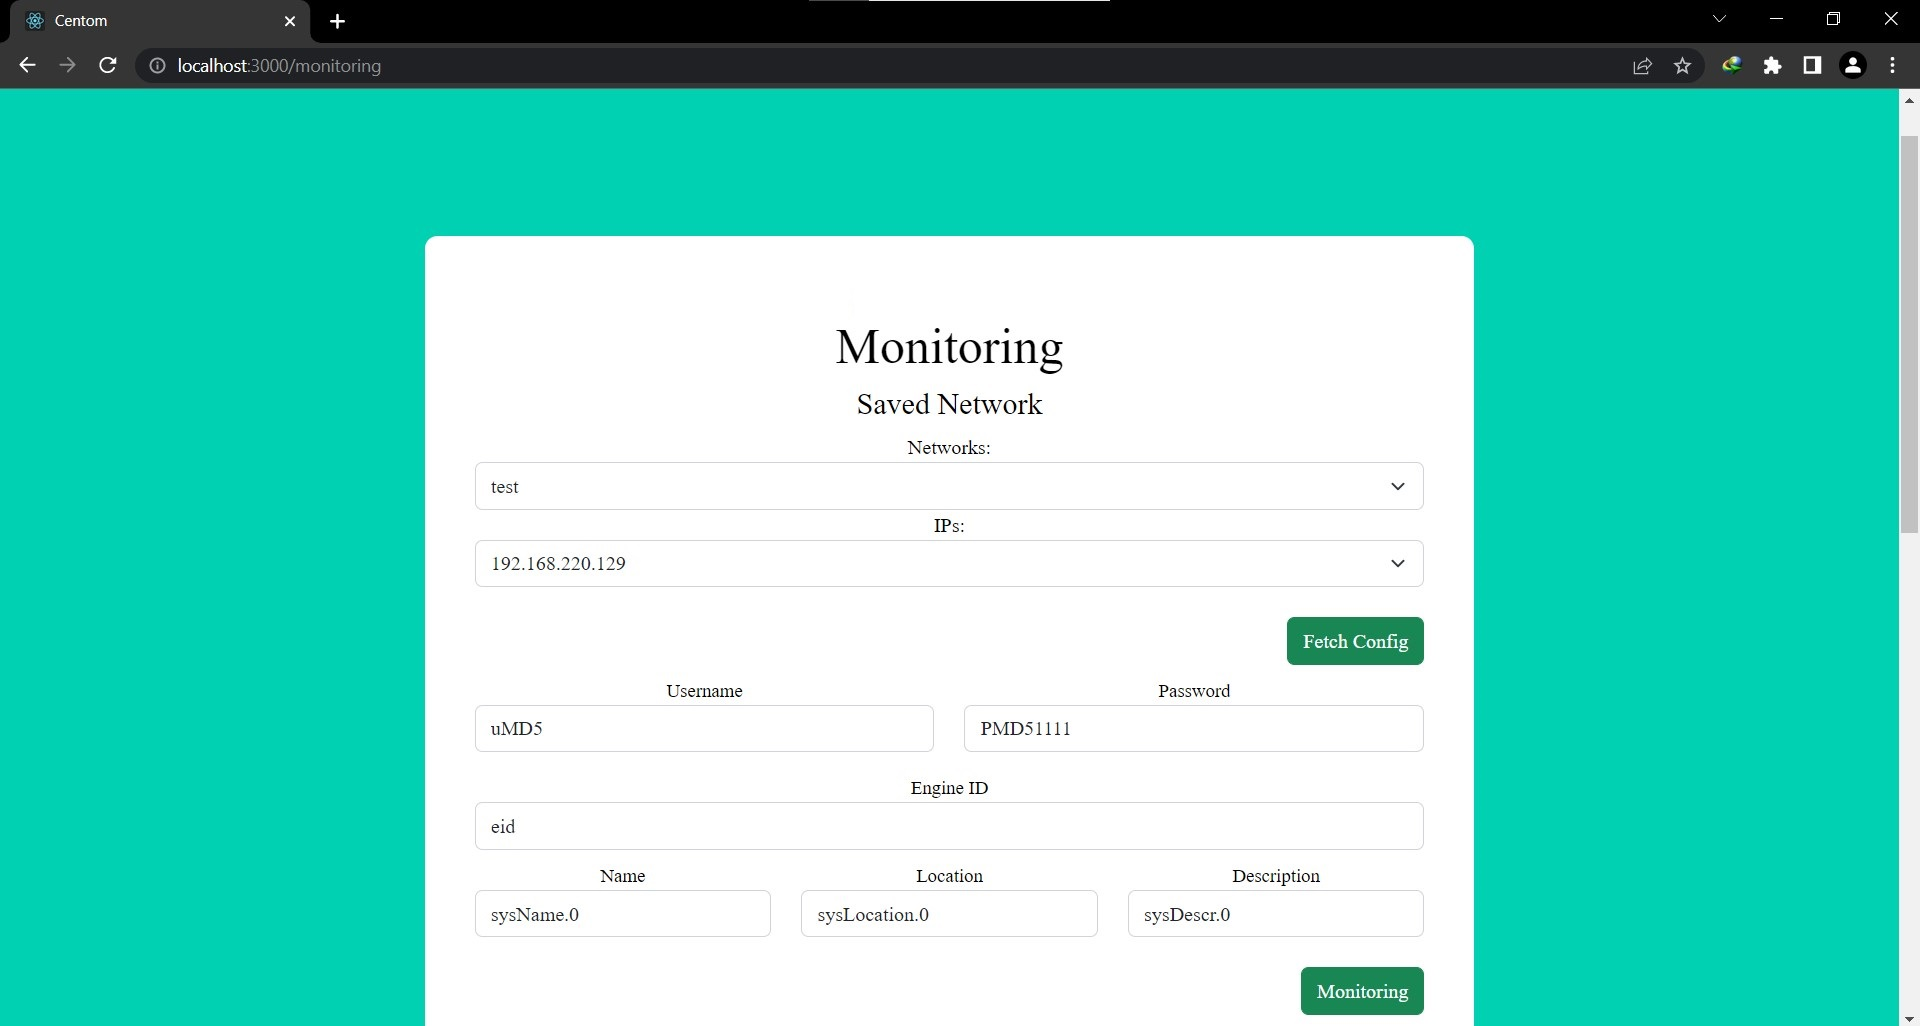
\includegraphics[scale=.38]{./monitoring}
    \caption{صفحه پایش شبکه}\label{fig.18}
\end{figure}


% نوتیفیکیشن //////////////////////////////////////////////////////////////////////////////////////////////////////

بعد از گزینه صفحه پایش، طبق معماری سامانه، صفحه اعلانات طبق \cref{fig.19} قرار دارد. در این صفحه پس از فشردن دکمه مورد نظر، سامانه به پورت 162 گوش می‌دهد و تله‌های دریافتی را در قالبی خوانا به مدیر نمایش می‌دهد.

\begin{figure}[!h]
    \centering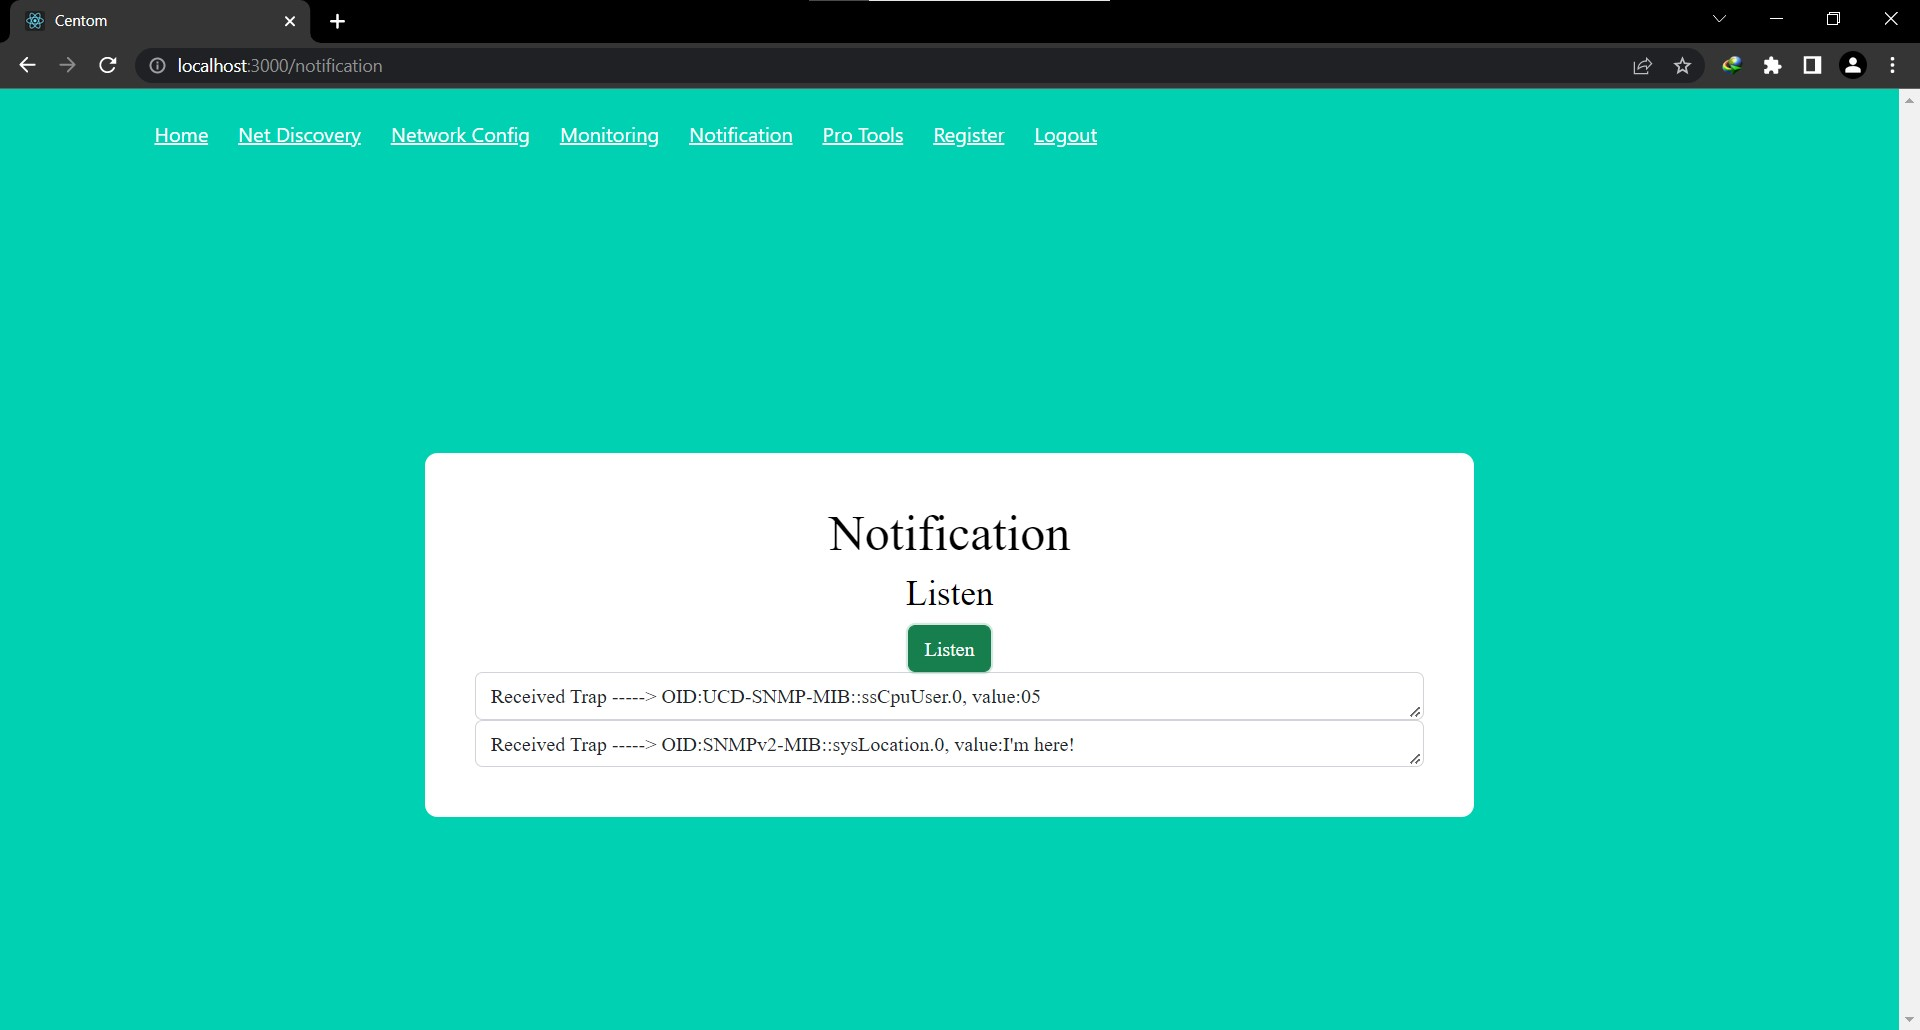
\includegraphics[scale=.38]{./notification}
    \caption{صفحه اعلانات دریافتی از شبکه}\label{fig.19}
\end{figure}

\cleardoublepage

در نهایت صفحه ابزارهای پیشرفته قرار دارد، که در حال حاضر تنها اسکن سریع آن در \cref{fig.120} موجود است. سامانه در این قسمت می‌تواند با دریافت یک آدرس و یک شناسه شی\LTRfootnote{\lr{Object Identifiers}}، پیام‌های \lr{get} و \lr{walk} را ارسال و نتیجه را به ترتیب مشاهده کند. 

\begin{figure}[!h]
    \centering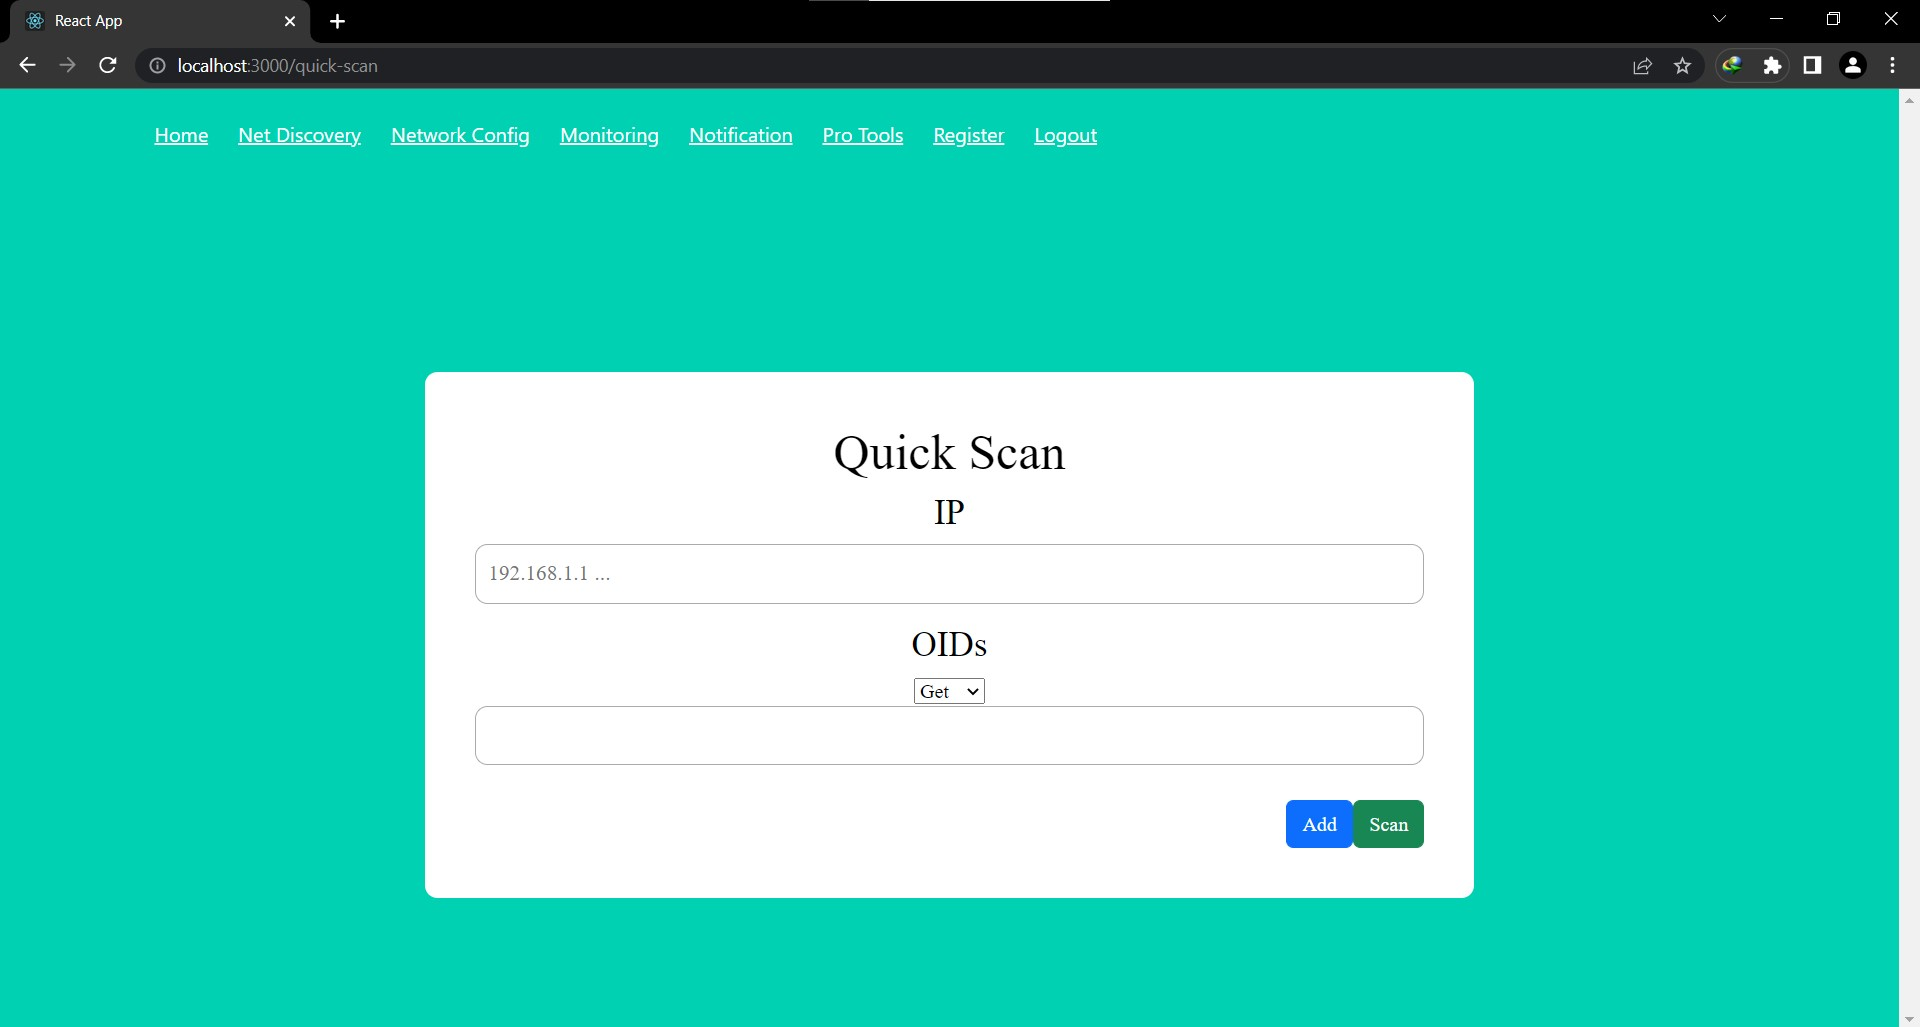
\includegraphics[scale=.38]{./pro-tools}
    \caption{صفحه ابزارهای پیشرفته}\label{fig.120}
\end{figure}



\cleardoublepage

\section{ذخیره‌سازی اطلاعات}

این دسته فقط شامل ماژول ذخیره‌سازی اطلاعات شبکه از \cref{fig.11} است. در این سامانه به طور کلی سه نوع داده کاربران، اطلاعات شبکه و اطلاعات دریافتی از عناصر تحت مدیریت شبکه وجود دارد\cite{Mirfendereski_Centom}.



\subsection{ذخیره‌سازی اطلاعات شبکه و کاربران}

برای ذخیره‌سازی اطلاعات کاربران و اطلاعات شبکه از پایگاه داده \lr{SQLite} با تعریف جدول‌ها شکل \cref{fig.121} استفاده می‌کنیم.

\begin{figure}[!h]
    \centering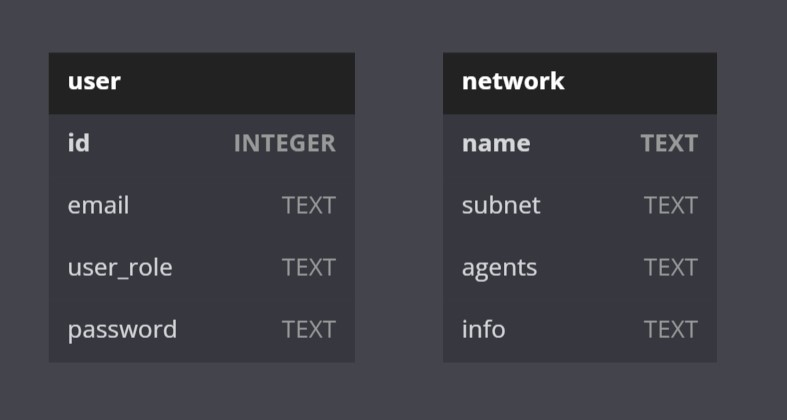
\includegraphics[scale=.60]{./db}
    \caption{تصویر جدول‌های تعریف شده در پایگاه داده \lr{SQLite}}\label{fig.121}
\end{figure}


فیلدهایی که نیاز است توضیحی درباره آن‌ها داده شود به صورت زیر است:

\begin{itemize}
    \item \lr{user-role}: نقش هر کاربر جهت دسترسی ‌های متنوع به سامانه را می‌دهد. به عنوان مثال مدیر ارشد به همه امکانات، مدیر معمولی به همه امکانات به جز ثبت‌نام کاربر جدید، تنظیمات و اسکن شبکه دسترسی دارند. و در نهایت کاربر عادی فقط به اسکن سریع یک دستگاه دسترسی خواهد داشت.
    \item \lr{name}: این فیلد فقط برای شناسایی متمایز شبکه‌ها کاربرد دارد. بدین صورت که با دریافت یک اسم از کاربر به هنگام ذخیره، تنها زمان بازیابی اطلاعات شبکه در سامانه کاربرد دارد.
    \item \lr{agents}: این فیلد شامل لیستی از دستگاه‌های شبکه است که عامل \lr{SNMP} بر روی آن‌ها فعال است.
    \item \lr{info}: این فیلد شامل شی‌ای از \lr{JSON}\LTRfootnote{\lr{JavaScript Object Notation}} شامل گره‌ها، یال‌ها و نوع دستگاه‌های تحت مدیریت است.

\end{itemize}


برای اتصال به پایگاه داده \lr{SQLite} نیز از \lr{SQLAlchemy} که یک ابزار نگاشت رابطه به شی\LTRfootnote{\lr{Object–relational mapping (ORM)}} است، استفاده شد که مزایای بسیاری دارد.



\subsection{ذخیره‌سازی اطلاعات دریافتی از شبکه}

این اطلاعات در درجه اول شامل پارامتر‌های مختلف جهت پایش دستگاه‌ها به همراه نرخ نمونه‌برداری\LTRfootnote{\lr{rate}} آن‌ها است. در درجه بعد شامل اطلاعات دریافتی از دستگاه‌های تحت مدیریت مربوط به پارامترهای مختلف خواهد بود. به علت تعداد بالای بازیابی این گونه اطلاعات از ردیس استفاده شد. برای اتصال به ردیس نیز از ماژول ردیس در پایتون استفاده شد.

\newpage

\section{سمت سرور}

این دسته شامل ماژول‌های پردازش اطلاعات شبکه، هشدار، کشف شبکه و جمع‌آوری اطلاعات (پایش) از \cref{fig.11} است. ادامه این فصل به بررسی ماژول‌های گفته شده می‌پردازد.


\subsection{ماژول کشف شبکه}

در این ماژول با توجه به نیازمندی‌های گفته شده در فصل تحلیل و طراحی، سامانه باید قادر باشد تا با دریافت یک آدرس شبکه، عناصری که عامل \lr{SNMP} بر روی آن‌ها فعال هستند را به همراه نوع عنصر (سرور، مسیریاب، سوییچ و تکرارکننده) آن‌ها مشخص کند. این خروجی باید بر اساس یک توپولوژی شبکه باشد.


این مسئله با توسعه یک الگوریتم مشخص باید حل شود. در ادامه تکنیک‌های موجود برای حل این مسئله بیان و بررسی می‌شوند. در نهایت نیز راه حل به کار گرفته شده ارائه می‌شود.

تکنیک‌های حل این مسئله:

\begin{itemize}
    \item استفاده از پینگ\LTRfootnote{\lr{Ping}} همه پخشی\LTRfootnote{\lr{Broadcast}} برای شناسایی تمام عناصر شبکه
    \item استفاده از پروتکل‌های کشف لایه پیوند\LTRfootnote{\lr{Link Layer Discovery Protocol (LLDP)}} و یا کشف سیسکو\LTRfootnote{\lr{Cisco Discovery Protocol (CDP)}}
    \item استفاده از پیام \lr{SNMP} با شناسه شی \lr{sysServices.0}
\end{itemize}

به علت عدم پشتیبانی بعضی از دستگاه‌ها از پروتکل‌های کشف لایه پیوند و کشف سیسکو و یا نیاز به ابزارهایی اضافی جهت حل این مسئله، از این دو پروتکل استفاده نشد. اما الگوریتمی که برای این مسئله توسعه داده شد به شرح زیر می‌باشد\cite{Mirfendereski_Centom}:

\begin{enumerate}
    \item ارسال یک پیام \lr{SNMP} با شناسه شی \lr{ sysServices.0} به تمام آدرس‌های موجود در آدرس شبکه (اگر پاسخی دریافت شود یعنی عنصر نیازمند مدیریت است.)
    \item رمز گشایی مقدار مرحله قبل در صورت دریافت پاسخ از آدرس مربوطه به صورت زیر:
    \begin{enumerate}
        \item تبدیل عدد برگردانده شده به فرمت باینری و تعیین نوع عنصر بر اساس مقادیر بیت‌ها (کم ارزش ترین بیت، بیت اول در نظر گرفته می‌شود)
        \item اگر بیت اول تنظیم شده باشد، دستگاه موردنظر یک نوع تکرارکننده است.
        \item اگر بیت دوم تنظیم شده باشد، دستگاه موردنظر یک نوع سوییچ است.
        \item اگر بیت سوم تنظیم شده باشد و همچنین مقدار پیام \lr{SNMP} با شناسه شی \lr{ ipForwarding.0 } یک باشد، دستگاه موردنظر یک نوع مسیریاب است.
        \item اگر هیچ کدام از موارد بالا نباشد و همچنین بیت چهارم یا هفتم تنظیم شده باشد، دستگاه موردنظر یک نوع سرور است.
        \item اگر مقدار برگردانده شده در موارد بالا صدق نمی‌کرد، نوع دستگاه متفرقه\LTRfootnote{\lr{Other}} خواهد بود (مثل یک دستگاه منبع تغذیه اضطراری\LTRfootnote{\lr{Uninterruptible Power Supply (UPS)}}). 
    \end{enumerate}
    \item به ازای تمام آدرس‌هایی که عامل \lr{SNMP} بر روی آن‌ها در حال اجرا هستند، دستور \lr{traceroute} اجرا می‌شوند. خروجی بدین صورت خواهد بود که تا رسیدن به مقصد نهایی گام‌های میانی نمایش داده می‌شوند. بدین ترتیب به تعداد عناصر فعال، مسیرهای رسیدن تا آن‌ها بدست می‌آیند.
    \item در نهایت برای رسم توپولوژی شبکه تحت یک گراف، با داشتن گره‌ها و همچنین یال‌های بدست آمده از مسیرها این امر ممکن می‌شود.
\end{enumerate}




\subsection{ماژول پردازش اطلاعات شبکه}

در این ماژول اطلاعات دریافت شده از سمت دستگاه‌های شبکه یعنی همان پیام‌های \lr{SNMP}، با توجه به مقدار آن‌ها پردازش می‌شوند. این پردازش شامل دو قسمت یعنی ابتدا نوع داده دریافتی را مشخص کرده و بعد از در صورت نیاز به حذف تعدادی کاراکتر از آن، اقدام می‌شود. قسمت دوم این پردازش بدین جهت خواهد بود که به عنوان مثال بعضی مقادیر حجم حافظه و ... در انتها عبارت \lr{KB} وجود دارد.

\subsection{ماژول جمع‌آوری اطلاعات }

برای راحتی انجام پایش و تنظیمات شبکه توسط سامانه، در پروژه یک فایل با پسوند \lr{JSON} طبق \cref{fig.122} تعبیه شده است. در این فایل دو نوع کلید وجود دارد. اولین کلید، پارامترهای پیش‌فرض\LTRfootnote{\lr{def\_params}} است. اهمیت بعضی پارامترها باعث اضافه شدن این بخش شد تا این پارامترها برای تمام دستگاه‌ها بدون نیاز به افزودن توسط مدیر ارشد رصد شوند. در ادامه هر کلید متعلق به این کلید، برای یک پارامتر به خصوص شامل شناسه شی، نرخ نمونه‌برداری و نحوه پردازش آن برای نمایش است. ساختار زیرین دومین کلید یعنی پارامترها\LTRfootnote{\lr{params}} نیز به همین صورت است. با این تفاوت که به مدیر ارشد لیستی از این موارد نشان داده شده و او می‌تواند برای هر \lr{IP} در بخش تنظیمات شبکه از این لیست انتخاب نماید. در ادامه نیز برای ارسال اطلاعات به صورت بی‌درنگ\LTRfootnote{\lr{real-time}} از \lr{SSE}\LTRfootnote{\lr{Server-Sent Events}} استفاده شد. که توسعه آن در فلسک و ری‌اکت کمی با چالش نیز همراه بود\cite{Mirfendereski_Centom}.


\begin{figure}[!h]
    \centering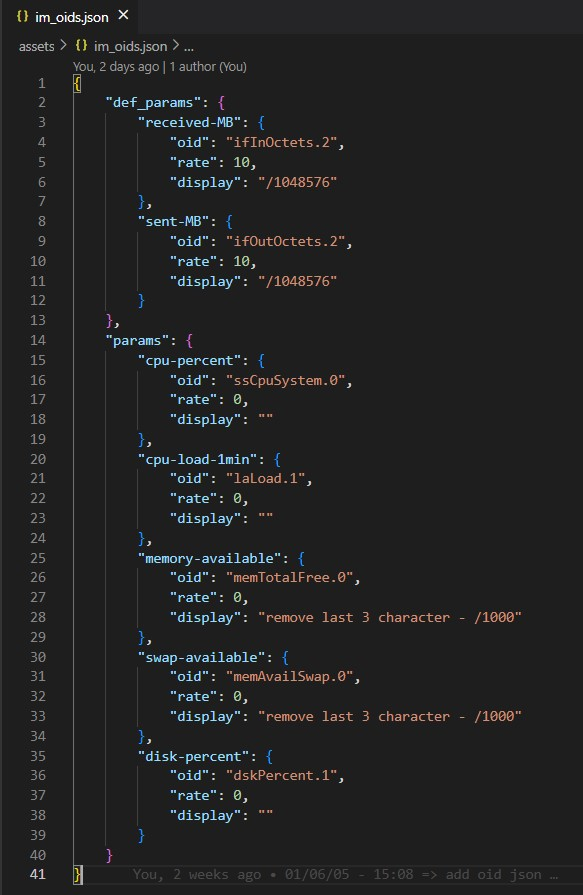
\includegraphics[scale=.80]{./im-json}
    \caption{تصویر فایل \lr{JSON} جهت مدیریت پارامترها}\label{fig.122}
\end{figure}




\subsection{ماژول هشدار}

ماژول هشدار که در قالب کلاس تله وظیفه خود را انجام می‌دهد. این ماژول باید دریافت اطلاعات و تفسیر آن‌ها کار خود را انجام دهد. همچنین اشاره به این نکته که تمام پیام‌های \lr{SNMP} با \lr{asn.1}\LTRfootnote{\lr{Abstract Syntax Notation One}} کدگذاری\LTRfootnote{\lr{encode}} و ارسال می‌شوند، لازم است. در واقع کاری که کلاس تله انجام می‌دهد را می‌توان به صورت مراحل زیر بیان کرد\cite{Mirfendereski_Centom}:

\begin{enumerate}
    \item گوش دادن به پورت 162 و دریافت اطلاعات
    \item تبدیل اطلاعات در قالب هگزادسیمال\LTRfootnote{\lr{hexadecimal}} به فرمت رشته\LTRfootnote{\lr{String}} در زبان \lr{C++}
    \item حذف کاراکترهای فاصله در رشته
    \item کدگشایی\LTRfootnote{\lr{decode}} رشته مورد نظر با \lr{asn.1} از طریق ابزارهای \lr{xxd} و \lr{openssl}

\end{enumerate}


\section{خلاصه}

این فصل با توجه به معماری طراحی شده در فصل قبل، با گروه‌بندی ماژول‌ها، نحوه پیاده‌سازی هر ماژول بیان شد. در ابتدا نحوه پیاده‌سازی هسته \lr{SNMP} بیان شد. بعد از آن به توضیح پیاده‌سازی واسط کاربری پرداخته شد. در ادامه نیز ذخیره‌سازی اطلاعات و درنهایت سمت سرور توضیح داده شدند. بخش سمت سرور نیز خود از چندین ماژول پردازش اطلاعات شبکه، هشدار، کشف شبکه و جمع‌آوری اطلاعات (پایش) تقسیم شده و به هرکدام به تفکیک پرداخته شد.